\section{Übung - JSON}
\label{sec:uebung_10}
Lese die Datei \texttt{orderdata.sql} aus dem Verzeichnis \texttt{data} ein. Diese legt die unten aufgeführte Tabelle weborders an, in der Kundenbestellungen im JSON-Format gespeichert werden.

\begin{figure}[H]
  \centering
  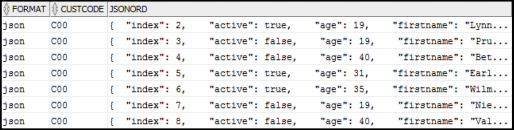
\includegraphics[width=1\textwidth]{img//uebung_10_-_vorbereitung.png}
  \label{img:uebung_10_-_vorbereitung}
\end{figure}

Jedes JSON-Dokument, in der Spalte jsonord, besitzt folgenden Aufbau:
\inputjson{./data/uebung_10_-_vorbereitung.json}

% ##########################################################################
% ############################### Aufgabe 01 ###############################
% ##########################################################################
\subsection{Aufgabe}
\label{sec:uebung_10.aufgabe_01}
Erzeuge folgende Bestellübersicht, in der nur Bestellungen aus 2014 berücksichtigt werden.

\begin{table}[H]
  \centering
  \ttfamily
  \begin{tabular}{|l|l|l|l|}
    \hline
    \textbf{FIRST}  & \textbf{LAST}   & \textbf{GEND} & \textbf{PHONE}      \\
    \hline
    Lakeisha Wood   & Cameron         & female        & +1 (914) 536-2858   \\
    Jenifer Silva   & Sexton          & female        & +1 (932) 510-3597   \\
    Wright Cate     & Simmons         & male          & +1 (978) 575-3520   \\
    Lynn May        & Mardin          & male          & +1 (988) 582-3186   \\
    Ruitt Hays      & Mann            & male          & +1 (965) 502-3118   \\
    Wilma Sparks    & Vega            & female        & +1 (861) 454-3116   \\
    \hline
  \end{tabular}
\end{table}

% ############################### Aufgabe 01A #############################
\subsubsection{Aufgabe}
\label{sec:uebung_10.aufgabe_01a}
Mithilfe der Funktion json\_value().

\paragraph*{Lösung}
\label{sec:uebung_10.aufgabe_01a.loesung}
\inputsql{./loesungen/uebung_10/uebung_10_-_aufgabe_01a.sql}


% ############################### Aufgabe 01B #############################
\subsubsection{Aufgabe}
\label{sec:uebung_10.aufgabe_01b}
Mithilfe der Funktion json\_table().

\paragraph*{Lösung}
\label{sec:uebung_10.aufgabe_01b.loesung}
\inputsql{./loesungen/uebung_10/uebung_10_-_aufgabe_01b.sql}


% ##########################################################################
% ############################### Aufgabe 02 ###############################
% ##########################################################################
\subsection{Aufgabe}
\label{sec:uebung_10.aufgabe_02}
Erzeuge folgende Übersicht, die alle Bestellpositionen darstellt.

\begin{table}[H]
  \centering
  \ttfamily
  \begin{tabular}{|l|l|l|r|r|}
    \hline
    \textbf{LAST} & \textbf{GEND} & \textbf{PHONE}    & \textbf{PROD\_ID} & \textbf{QUANT}  \\
    \hline
    Mann          & male          & +1 (965) 502-3118 & 2323              & 59              \\
    Mann          & male          & +1 (965) 502-3118 & 2321              & 55              \\
    Mann          & male          & +1 (965) 502-3118 & 2393              & 21              \\
    Mann          & male          & +1 (965) 502-3118 & 2337              & 37              \\
    Mann          & male          & +1 (965) 502-3118 & 1763              & 25              \\
    Mann          & male          & +1 (965) 502-3118 & 2308              & 22              \\
    Mann          & male          & +1 (965) 502-3118 & 1763              & 28              \\
    Mann          & male          & +1 (965) 502-3118 & 2311              & 43              \\
    English       & female        & +1 (947) 528-3476 & 2359              & 36              \\
    English       & female        & +1 (947) 528-3476 & 1772              & 44              \\
    English       & female        & +1 (947) 528-3476 & 1772              & 25              \\
    \hline
  \end{tabular}
\end{table}

\subsection*{Lösung}
\label{sec:uebung_10.aufgabe_02.loesung}
\inputsql{./loesungen/uebung_10/uebung_10_-_aufgabe_02.sql}


% ##########################################################################
% ############################### Aufgabe 03 ###############################
% ##########################################################################
\subsection{Aufgabe}
\label{sec:uebung_10.aufgabe_03}
Erzeuge eine Übersicht, die für alle Webkunden die abgesetzte Menge je aktivem und nicht aktivem Mitglied sowie die insgesamt abgesetzte Menge zurückgibt.

\begin{table}[H]
  \centering
  \ttfamily
  \begin{tabular}{|l|r|}
    \hline
    \textbf{ACTIVE} & \textbf{SUM\_QUANT} \\
    \hline
    false           & 5889                \\
    true            & 4123                \\
    (null)          & 10012               \\
    \hline
  \end{tabular}
\end{table}

\subsection*{Lösung}
\label{sec:uebung_10.aufgabe_03.loesung}
\inputsql{./loesungen/uebung_10/uebung_10_-_aufgabe_03.sql}


% ##########################################################################
% ############################### Aufgabe 04 ###############################
% ##########################################################################
\subsection{Aufgabe}
\label{sec:uebung_10.aufgabe_04}
Gebe für jeden Monat im Jahr 2015 die Top-2 Webkunden aus, die die meisten Produkte bestellt haben.

\begin{figure}[H]
  \centering
  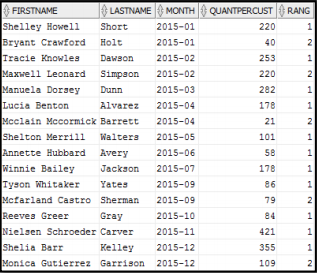
\includegraphics[width=0.6\textwidth]{img//uebung_10_-_aufgabe_04.png}
  \label{img:uebung_10_-_aufgabe_04}
\end{figure}

\subsection*{Lösung}
\label{sec:uebung_10.aufgabe_04.loesung}
\inputsql{./loesungen/uebung_10/uebung_10_-_aufgabe_04.sql}


% ##########################################################################
% ############################### Aufgabe 05 ###############################
% ##########################################################################
\subsection{Aufgabe}
\label{sec:uebung_10.aufgabe_05}
Zeige für jeden Webkunden die Anzahl der insgesamt georderten Bestellpositionen.

\subsection*{Lösung}
\label{sec:uebung_10.aufgabe_05.loesung}
\inputsql{./loesungen/uebung_10/uebung_10_-_aufgabe_05.sql}
